\chapter{Business Understanding}
Questa fase si focalizza sulla individuazione degli obiettivi e i requisiti del progetto dal punto di vista del business. Per fare ciò, si è deciso di utilizzare prettamente la documentazione allegata al dataset.

\begin{figure}[hbtp]
	\centering
	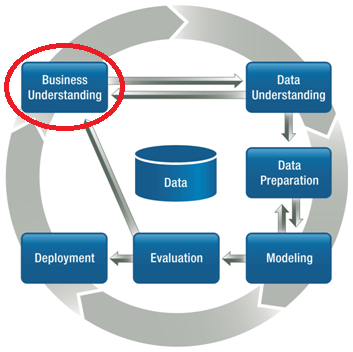
\includegraphics[width=0.5\textwidth]{./images/CRISPDM_1.png}
	\caption{CRISP-DM - Business Understanding}
	\label{CRISPDM_1}
\end{figure}

\section{Background}\label{Background}
Ogni giorno, vengono inviate circa 25 milioni di email indesiderate, chiamate anche email di spam. Tale cifra corrisponde a quasi il 10 \% di tutte le email inviate nel mondo; inoltre, indagini svolte sull'argomento, rivelano che generalmente il 40 \% delle email ricevute giornalmente dai dipendenti di molte imprese risultano essere email di spam, arrivando in alcuni casi, anche al 90 \%.
Queste percentuali risultano essere molto elevate principalmente a causa della facile diffusione delle proprie caselle di posta verso qualunque tipo di contatto, diventando cosi bersagli di messaggi promozionali di qualunque tipo. Questa sovraccarico di spam genera principalmente due problemi:
\begin{itemize}
\item Saturazione della propria casella di posta, anche se al giorno d'oggi si dispone di una capienza elevata;
\item Perdita di tempo abbastanza considerevole da parte del ricevente nel filtrare queste email.
\end{itemize}
Nel corso degli anni, il desiderio di automatizzare il rilevamento e relativa selezione di queste email di spam, ha portato alla creazione e diffusione di numerosi progetti software e di prodotti commerciali in grado di filtrare lo spam in maniera tutto sommato efficiente; uno dei più diffusi è \textit{SpamAssassin} \footnote{\url{http://spamassassin.apache.org/}}, programma opensource rilasciato sotto licenza Apache 2.0. Si basa su regole di confronto del contesto, ma supporta anche regole basate su DNS, checksum e filtraggio statistico, inoltre supporta programmi esterni e database online.
SpamAssassin è considerato uno dei filtri antispam più efficaci, specialmente se usato congiuntamente con un database antispam.\cite{wiki:SpamAssassin}

\subsection{Risorse}
La principale risorsa in uso è l'hardware del sistema utilizzato per eseguire l'algoritmo di data mining, in particolar modo, un sistema Windows con un Quad-Core Intel i7 2.00 GHz avente 4 GB di Ram.
Il tool di data mining scelto è WEKA (\textbf{W}aikato \textbf{E}nvironment for \textbf{K}nowledge \textbf{A}nalysis) \cite{WEKA}:
una popolare suite di software per il machine learning scritta in Java sviluppata dall'Università di Waikato (Nuova Zelanda); è stato deciso di utilizzare tale suite, in quanto il software porta con sè i seguenti vantaggi :
\begin{itemize}
	\item Liberamente scaricabile dal sito \footnote{Weka site: \url{http://www.cs.waikato.ac.nz/ml/weka/downloading.html}};
    \item Portabile, in quanto totalmente implementato in java;
    \item Ampia gamma di tecniche di preprocessing e modellazione dei dati;
    \item Facile da usare grazie alla GUI;
\end{itemize}
Per quanto riguarda invece il personale umano, l'unica risorsa umana interpellata nella sperimentazione è lo sperimentatore stesso.
\subsection{Vincoli}
	Non sono presenti nè vincoli temporali, nè problemi legali legati alla diffusione del dataset in questione.
\subsection{Assunzioni}
	Si assume che i dati di cui si intende disporre siano liberamente accessibili e che non siano falsi o errati.
\section{Obiettivi di Business}
	Secondo quanto detto in precedenza, l'obiettivo di business di questo progetto consiste nell'individuazione delle email di spam attraverso l'utilizzo di tecniche di Data Mining.

\subsection{Task di Data Mining}
	\label{task}
	Il task da realizzare è di tipo \textit{predittivo}, in particolar modo, sarà un task di \textit{classificazione}. L'obiettivo sarà quindi quello di creare un classificatore che sia in grado di etichettare correttamente le nuove email come \textit{spam} o \textit{nospam} sulla base del training set dato in pasto al classificatore. 

\section{Criteri di successo}
	Il processo di KDD andrà a buon fine qualora siano rispettate due condizioni:
	\begin{itemize}
		\item 	Nel set di email ottenute dopo aver effettuato il filtraggio, potranno essere ammesse fino ad un massimo dell'1 \% di email di spam;
				%Nel risultato del filtraggio, il numero di email di spam deve essere limitato all' 1\% della totalità;
				%Condizione necessaria: filtrare le email con un massimo dell'1\% di spam accettato.				
		\item	Minimizzare il numero di messaggi di spam che passeranno attraverso il filtro.
	\end{itemize}

\section{Glossario dei termini}
\textbf{Messaggi di spam}: "\textit{Lo spamming, detto anche fare spam o spammare, è l'invio di messaggi indesiderati (generalmente commerciali). Può essere attuato attraverso qualunque sistema di comunicazione, ma il più usato è Internet, attraverso messaggi di posta elettronica, chat, tag board o forum.}" (cit. Wikipedia)\cite{wiki:Spam}

\section{Analisi Costi-Benefici}
Per quanto riguarda i costi inerenti al processo di KDD, l'unico costo che si avrà, sarà in termini di risorse temporali utilizzate per la realizzazione e relativa verifica dei risultati che il classificatore produrrà.
Invece, i benefici che si otterranno da questo processo, saranno quelli che andranno a sopperire a ciò che è stato detto in precedenza nel paragrafo \ref{Background}.

\section{Piano di Progetto}
Il piano di progetto prevede la realizzazione rigorosa delle fasi definite dal modello di processo CRISP-DM (figura \ref{CRISPDM}).
In particolar modo, per ogni fase del modello, verrà definito un report riassuntivo : 
\begin{figure}[hbtp]
	\centering
	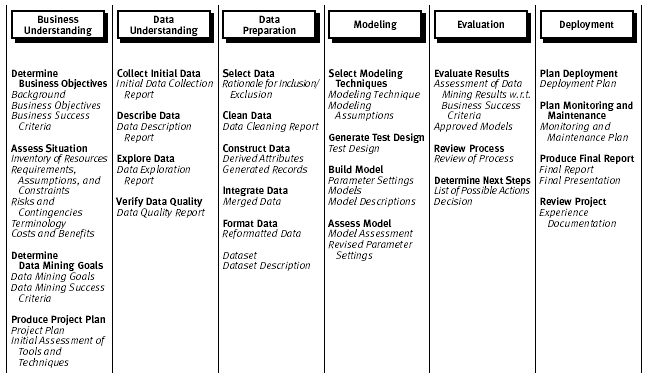
\includegraphics[width=1\textwidth]{./images/Metodologia_CRISP_DM.png}
	\caption{Report CRISP-DM}
	\label{Report_CRISPDM}
\end{figure}
Dal punto di vista di sforzo computazionale, oltre il 70 \% del tempo speso viene impiegato nella realizzazione delle fasi di \textit{Data Understanding} e di \textit{Data Preparation}, mentre il restante 30 \% per le fasi rimanenti.
Questo potrebbe portare alla necessità di dover rieseguire principalmente la fase di Data Preparation e, qualora i risultati dovessero dare esiti negativi, rieseguire anche la fase di Data Understanding in quanto ci potrebbero essere eventuali incomprensioni dei dati presi in considerazione.
Per quanto riguarda il tempo necessario a concludere il progetto, si prevede un massimo di tre settimane.